\subsection{The Heart-on-a-Chip platform}
\label{HoC}

\begin{figure}[!t]
	\centering
	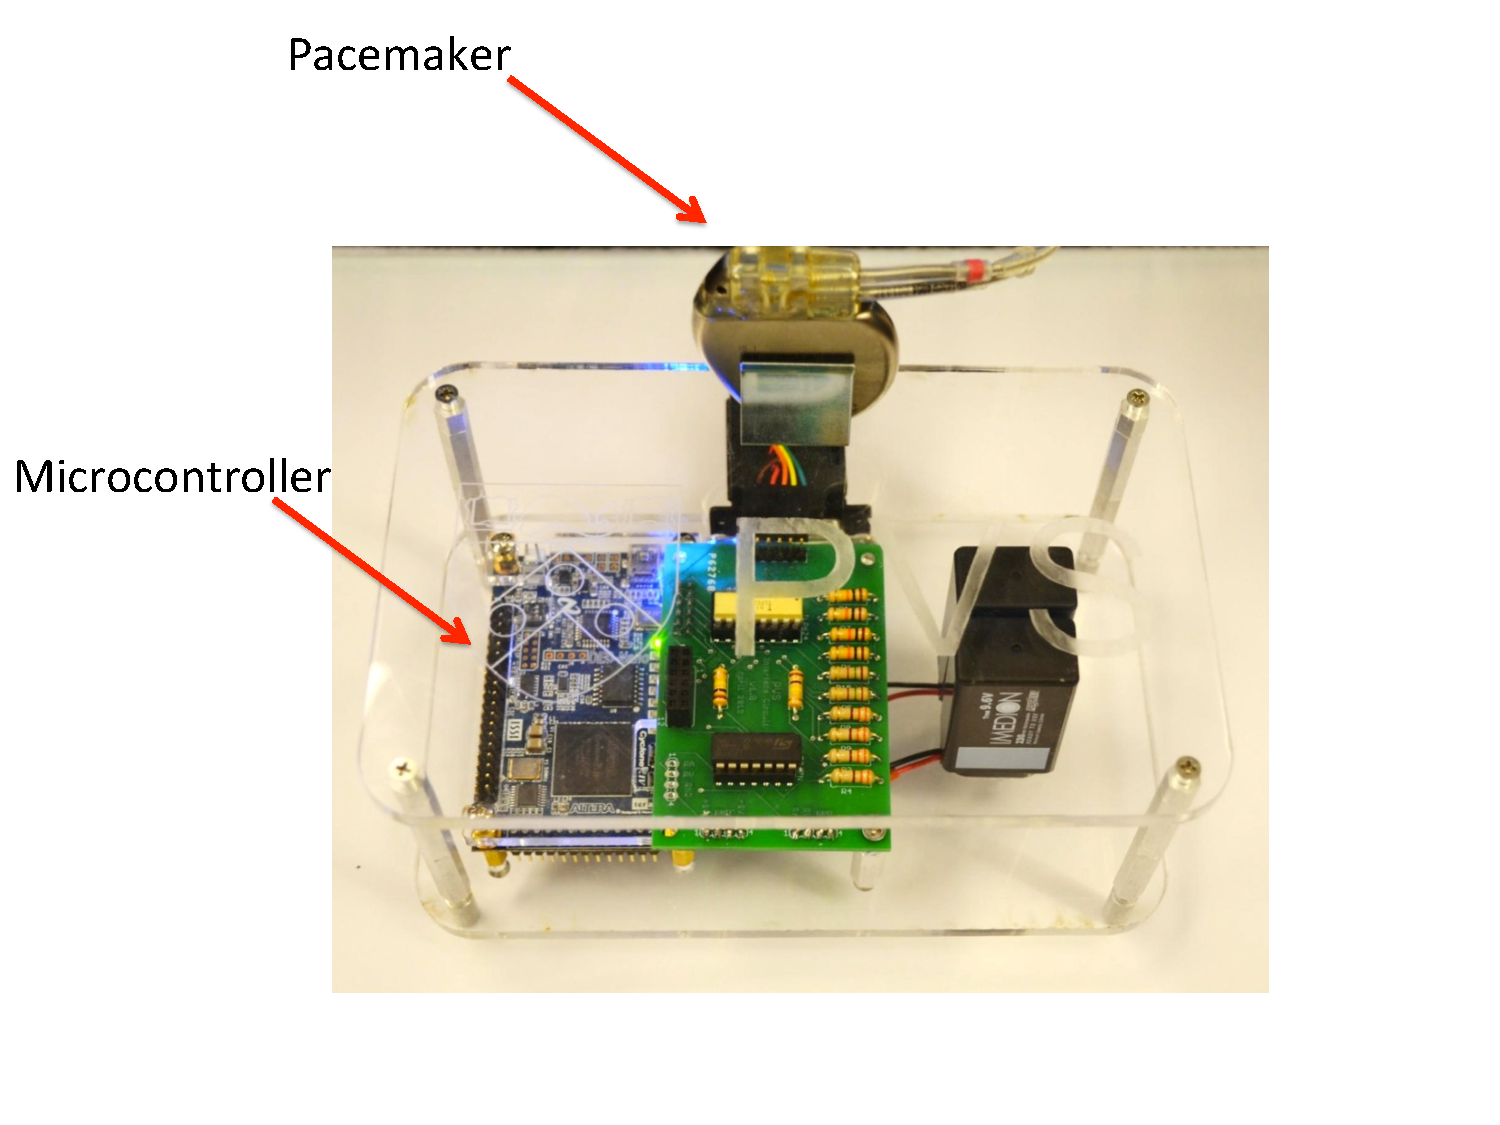
\includegraphics[scale=0.4]{HOCannotated.pdf}		
	\caption{\small Heart-on-a-Chip platform, showing the pacemaker, the microcontroller running the VHM code, and the monitors.}
	\label{fig:hoc}
\end{figure} 

Our closed-loop testing scheme ranges across different stages of the development process. 
In particular, it can be performed not only on pacemaker models and code, but also on off-the-shelf pacemaker devices. Fig.~\figref{hoc} shows the Heart-on-a-Chip (HoC) platform for closed-loop testing of pacemakers. 
The platform consists of a micro-controller running the code of the VHM, and an analog interface that converts heart signals
